\documentclass{article}
\usepackage[utf8x]{inputenc}
\usepackage[english,russian]{babel}
\usepackage{graphicx}
\usepackage{todonotes}
\usepackage{hyperref}
\usepackage{caption}
\begin{document}
\title{Изучение методов сейсмической миграции на примере волнового уравнения}
\author{\textbf{Голубев В.И., Войнов О.Я.} \\ Лаборатория прикладной вычислительной геофизики МФТИ}
\maketitle

\section{Введение}

Одним из методов поиска и разведки месторождений полезных ископаемых, таких как нефть и природный газ, является сейсморазведка.
Её основа - распространение упругих волн в геологических средах, а также их отражение от неоднородностей.
Как правило, в качестве источника сигнала используется взрывчатое вещество, расположенное на дневной поверхности.
Для регистрации сигнала используются сейсмоприёмники - специальные устройства, регистрирующие движения поверхности.

В дальнейшем на основе обработки накопленных данных делаются выводы о внутреннем строении геологической среды (мощности пластов,
зоны трещиноватости, границы резервуара).
При этом принято различать две задачи такой обработки: определение положения отражающих горизонтов (миграция) и восстановление скоростной модели среды (инверсия).

Перед авторами отчёта были поставлены следующие научно-технические задачи:
\begin{itemize}
\item изучение методов сейсмической миграции на примере волнового уравнения;
\item разработка вычислительного алгоритма и компьютерной программы миграции на основе интегральной формулы Кирхгофа;
\item разработка вычислительного алгоритма и компьютерной программы миграции на основе сопряженного оператора для волнового уравнения;
\item сравнительный анализ двух алгоритмов на простых моделях.
\end{itemize}

Все задачи были выполнены.

Лидер проекта – Василий Голубев.
Рекомендуемые руководителем лаборатории разделы книги “Geophysical inverse theory and regularization problems” - раздел 15.4 стр 503 - 516.

\section{Используемые обозначения}

Для ясности опишем кратко использованные и разработанные программные продукты.

KirScal - программа для расчёта интеграла Кирхгофа в трёхмерной постановке для волнового уравнения (однородная среда). Предполагается, что на верхней границе полупространства задаётся произвольный источник. Производится построение волнового поля в заданный момент времени. Разработана Голубевым В.И.

AcInverse - программа для построения миграционного изображения (волновое уравнение) с использованием формулы Кирхгофа (приближение Рэлея).
Разработана Голубевым В.И.

Borni - программа для решения прямой задачи (волновое уравнение) и построения миграционного изображения на основе подхода с присоединённым оператором.
При этом матрица связи наблюдений и параметров модели получена с использованием приближения Борна (частотная область).
Миграционное изображение строится на основе least-square migration.
Разработана Войновым О.Я.

Madagascar - OpenSource комплекс для моделирования/обработки данных сейсмической разведки.
Включает широкий спектр программ, как для прямого моделирования и построения синтетических сейсмограмм, так и для решения обратных задач (миграция, инверсия).
Разработка начата в 2003 году, проект актуален (например, Workshop August 2014).

\section{Теория}

Динамическое поведение акустической среды (распределение отклонения давления в ней от стационарного значения)
может быть описано следующим волновым уравнением (\cite{Zhdanov_2007}, 13.54):
\begin{equation}
\label{wave_equation}
\nabla^2P(\vec{r},t) - \frac{1}{c^2(\vec{r})}\frac{\partial^2}{\partial t^2}
	P(\vec{r},t) = - F^e(\vec{r},t),
\end{equation}

где - $P(\vec{r},t)$ - поле давления, $F^e(\vec{r},t)$ - напряжение внешнего источника, $c(\vec{r})$
- скорость распространения волны в среде.

\subsection{Решение прямой задачи. Интеграл Кирхгофа}

Рассмотрим задачу о воздействии динамического источника на поверхность некоторого объёма среды.
В этом случае значение давления во внутренней точке области $\vec{r'}$ в момент времени $t'$ может быть выражено следующей формулой (\cite{Zhdanov_2007}, 13.112):
\begin{equation}
\label{eq_kirchhoff_common}
P(\vec{r'}, t') = \int_S \int_{-\infty}^{+\infty} [G^w(\vec{r'}, t' | \vec{r}, t) \frac{\partial}
{\partial n} P(\vec{r}, t) - P(\vec{r}, t) \frac{\partial}{\partial n} G^w(\vec{r'}, t' |
\vec{r}, t)] dt ds,
\end{equation}

где интеграл берётся по поверхности, ограничивающей объём, а функция $G^w(\vec{r'}, t' | \vec{r}, t)$ называется функцией Грина и является решением уравнения \ref{wave_equation} для случая внешнего воздействия в виде дельта-функции.

Пусть $c(\vec{r'}) = const$, т.е. среда является изотропной.
Тогда функция Грина может быть получена аналитически (\cite{Zhdanov_1988}, 4.13):
\begin{equation}
\label{eq_grin_function}
G^w(\vec{r}, t | \vec{r'}, t') = \frac{1}{4\pi|\vec{r} - \vec{r'}|}\delta(t - t' - \frac{|\vec{r} -
\vec{r'}|}{c}),
\end{equation}
где $\vec{r'}, t'$ - место расположения источника и время, в которое он начал действовать.

Подставляя в (\ref{eq_kirchhoff_common}) выражение для функции Грина в явном виде (\ref{eq_grin_function}) получим
\begin{equation}
\label{eq_kirchhoff_homogeneous}
P(\vec{r'}, t') = \frac{1}{4\pi} \int_S [\frac{1}{c|\vec{r'} - \vec{r}|}
\frac{\partial |\vec{r'} - \vec{r}|}{\partial n}\frac{\partial P'}{\partial t'}
- \frac{\partial}{\partial n}(\frac{1}{|\vec{r'} - \vec{r}|}) P' + 
\frac{1}{|\vec{r'} - \vec{r}|}\frac{\partial}{\partial n}P'] ds,
\end{equation}
где $P' = P(\vec{r}, t' - \frac{|\vec{r'} - \vec{r}|}{c})$.
 
Для задач сейсмики актуальна задача о распространении сейсмических волн в полупространстве (от дневной поверхности вниз и обратно после отражения от неоднородностей).
При такой постановке $\frac{\partial}{\partial n} = -\frac{\partial}{\partial z}$, поэтому выражение (\ref{eq_kirchhoff_homogeneous}) может быть упрощено до вида:
\begin{equation}
\label{eq_kirchhoff_final}
P(\vec{r'}, t') = \frac{1}{4\pi} \int_S [\frac{z' - z}{|\vec{r'} - \vec{r}|}(\frac{1}{c}
\frac{\partial P'}{\partial t'} + \frac{1}{|\vec{r'} - \vec{r}|^2} P') - \frac{1}{|\vec{r'}
- \vec{r}|}\frac{\partial P'}{\partial z}] ds
\end{equation}

Пусть, например, дополнительно известна функция источника (импульс Риккера):
\begin{equation}
\label{eq_ricker_wavelet}
P_{ricker} = P_0(1-2 \pi^2f^2t^2)e^{-\pi^2f^2t^2}.
\end{equation}

Тогда могут быть явно вычислены производные, стоящие в выражении (\ref{eq_kirchhoff_final}):
\begin{equation}
\label{eq_dp'_dt'}
\frac{\partial P'}{\partial t'} = -2\pi^2f^2P_0(3-2 \pi^2f^2(t' - \frac{|\vec{r'} - \vec{r}|}{c})^2)e^{-\pi^2f^2(t' - \frac{|\vec{r'} - \vec{r}|}{c})^2},
\end{equation}
и
\begin{equation}
\label{eq_dp'_dz}
\frac{\partial P'}{\partial z} = -2\pi^2f^2P_0(t' - \frac{|\vec{r'} - \vec{r}|}{c})[3-2 \pi^2f^2(t' - \frac{|\vec{r'} - \vec{r}|}{c})^2]e^{-\pi^2f^2(t' - \frac{|\vec{r'} - \vec{r}|}{c})^2}
\frac{z'-z}{c|\vec{r'}-\vec{r}|},
\end{equation}
а функция $P'(\vec{r'}, t')$ может быть записана в виде:
\begin{equation}
\label{eq_surface_pressure}
P'(\vec{r'}, t') = P(\vec{r}, t' - \frac{|\vec{r'} - \vec{r}|}{c}) = P_0(1-2 \pi^2f^2(t' - \frac{|\vec{r'} - \vec{r}|}{c})^2)e^{-\pi^2f^2(t'-\frac{|\vec{r'} - \vec{r}|}{c})^2}.
\end{equation}

\subsection{Миграция. Интеграл Кирхгофа.}

В книге \cite{Zhdanov_2007} изложена теория, позволяющая рассчитать пространственное распределение скалярного параметра $U^m(\vec{r'})$, высокие значения которого соответствуют
месту расположения отражающего горизонта.
Для случая горизонтальной плоскости наблюдения расчётная формула представима в виде (\cite{Zhdanov_2007}, 15.208):
\begin{equation}
\label{rayleigh_migration}
U^m(\vec{r'}) = -\frac{1}{2\pi}\frac{\partial}{\partial z'}
	\int_S \frac{P(\vec{r},\frac{2|\vec{r'}-\vec{r}|}{c})}{|\vec{r'}-\vec{r}|}ds,
\end{equation}
где $\vec{r}$ - координата на поверхности, в которой записывается сейсмограмма, $\vec{r'}$ - координата в объёме, где ищется мигрированное изображение, $c$ - скорость распространения волн.

\subsection{Миграция. Приближение Борна.}

\todo[inline]{ОПИСАНИЕ ОТ ОЛЕГА ТЕОРИИ ПО БОРНУ}

\section{Численное моделирование}

\subsection{Решение прямой задачи. Интеграл Кирхгофа}

Была разработана программа KirScal на языке Python, которая вычисляет численно интеграл (\ref{eq_kirchhoff_final}) методом прямоугольников с подстановкой (\ref{eq_dp'_dt'} и \ref{eq_dp'_dz}).
Проведён расчёт с $C_P = 2000$ м/с, импульс Риккера с $f = 50$ Гц.
На рисунках (\ref{img_point_1} - \ref{img_point_3}) представлены волновые картины при воздействии точечного источника.
Как видно, происходит распространение сферической волны от места расположения источника вглубь среды.

\noindent
\begin{minipage}{\linewidth}
\makebox[\linewidth]{
  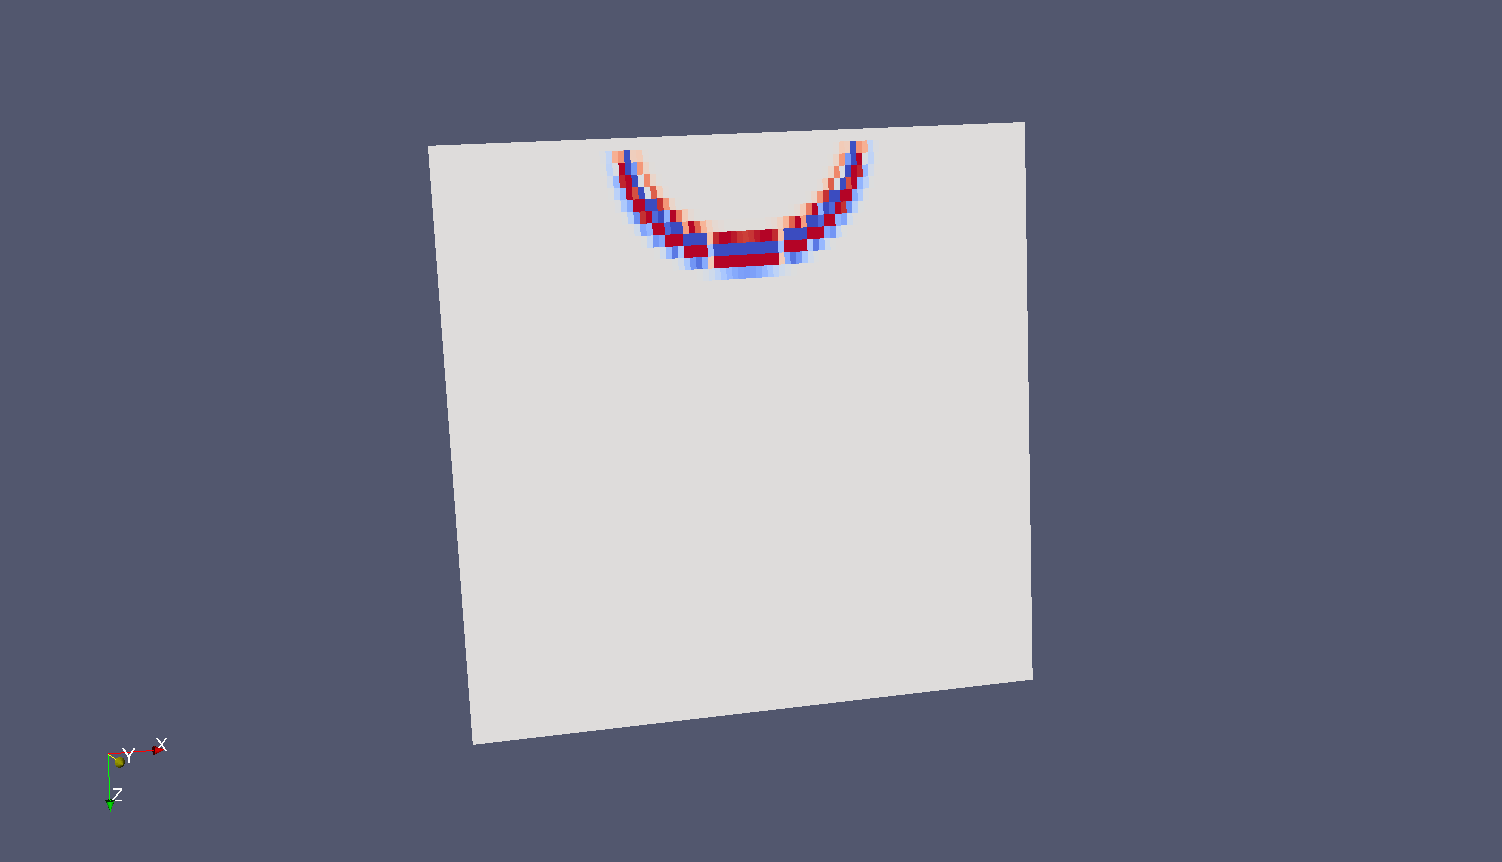
\includegraphics[scale=0.2]{pic_kirchhoff_scalar/point_1.png}
}
\captionof{figure}{Распределение давления по области через 100 мс}
\label{img_point_1}
\end{minipage}

\noindent
\begin{minipage}{\linewidth}
\makebox[\linewidth]{
    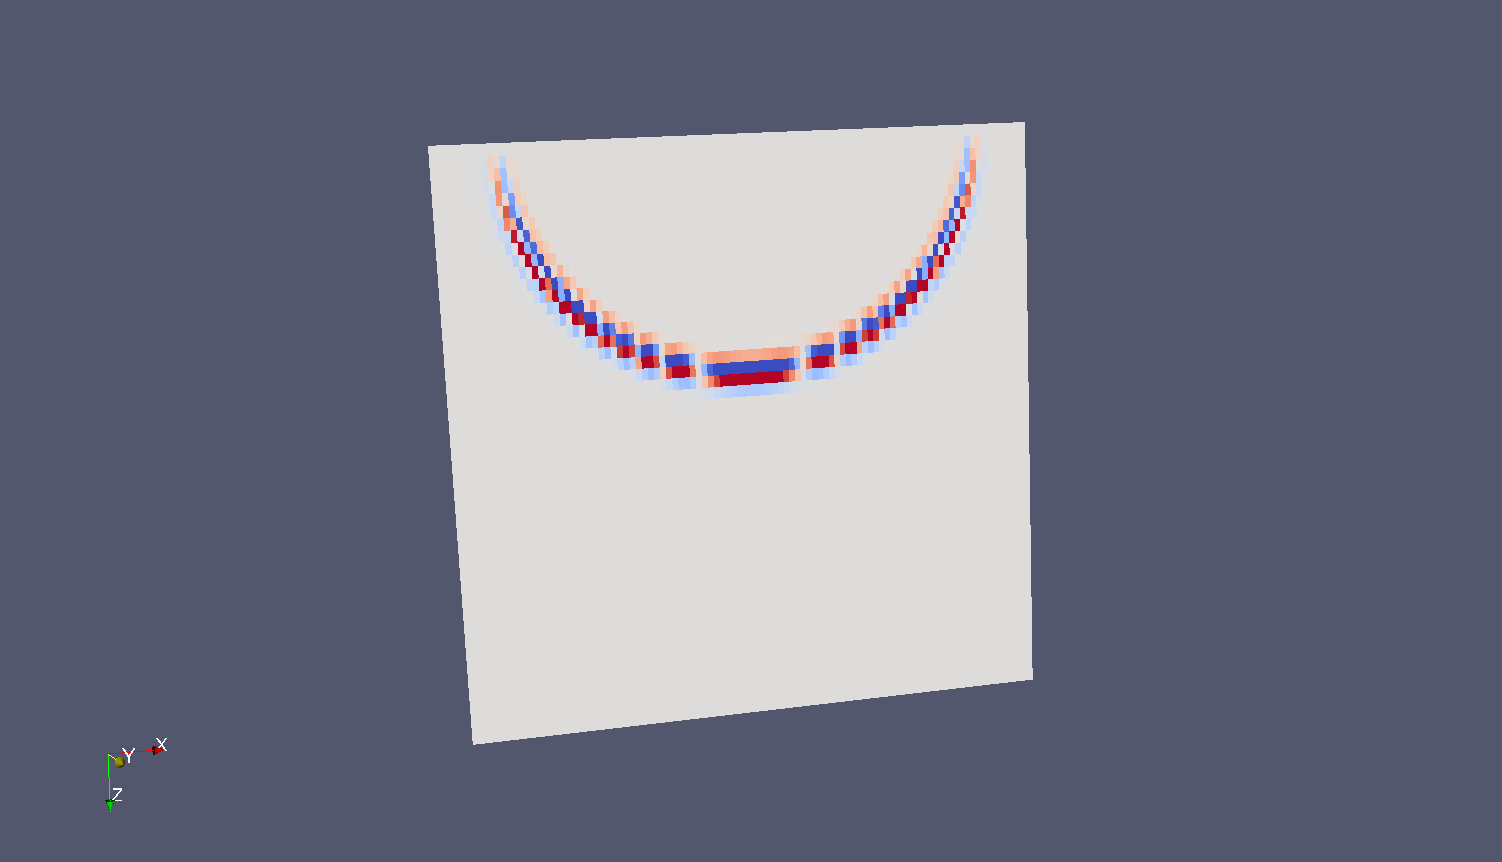
\includegraphics[scale=0.2]{pic_kirchhoff_scalar/point_2.png}
}
\captionof{figure}{Распределение давления по области через 200 мс}
\label{img_point_2}
\end{minipage}

\noindent
\begin{minipage}{\linewidth}
\makebox[\linewidth]{
  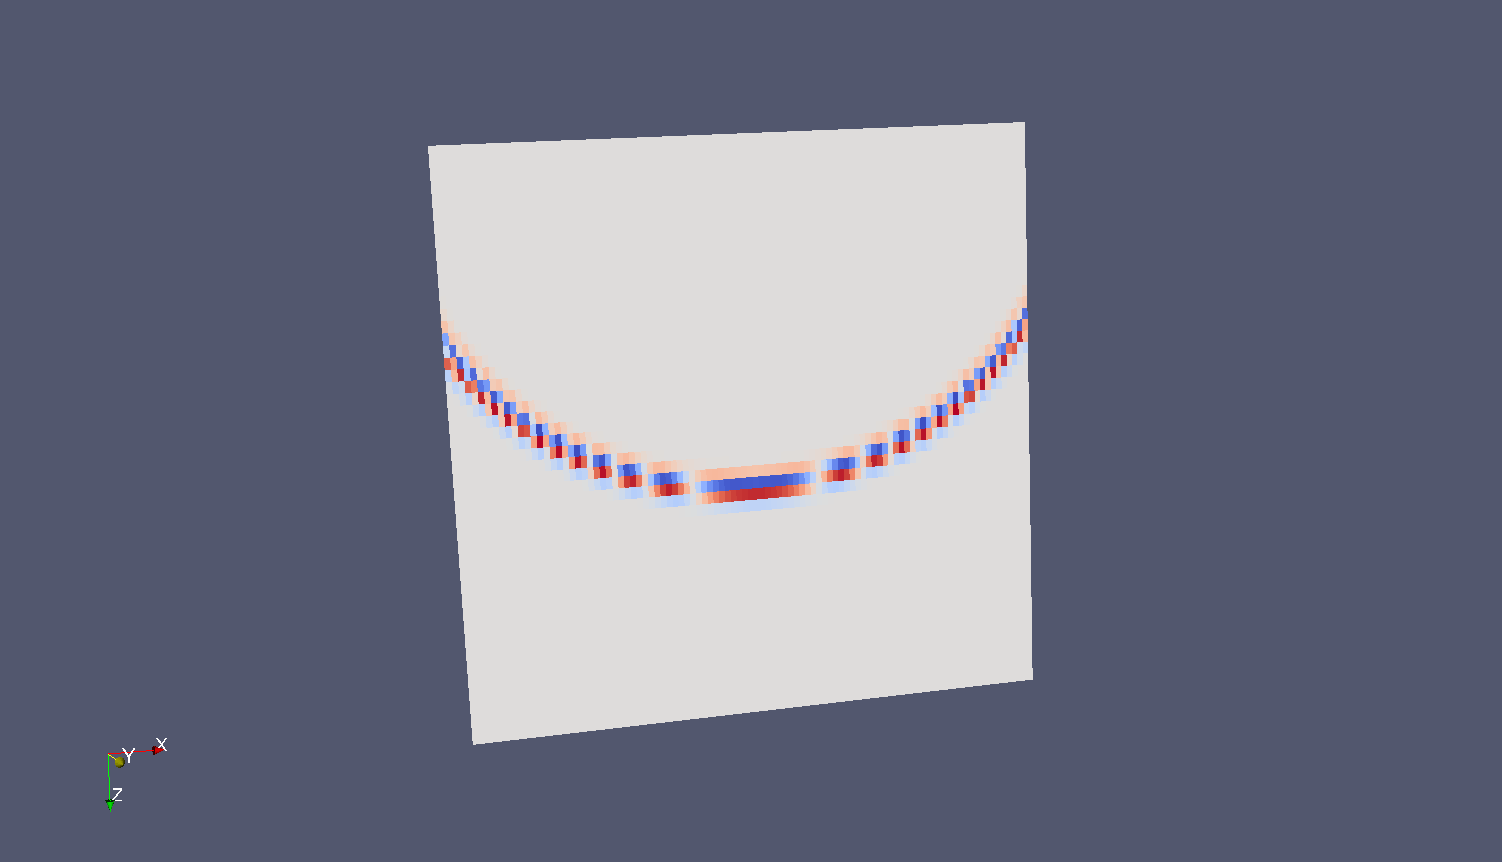
\includegraphics[scale=0.2]{pic_kirchhoff_scalar/point_3.png}
}
\captionof{figure}{Распределение давления по области через 300 мс}
\label{img_point_3}
\end{minipage}

\subsection{ПО Madagascar.}

Существует несколько программных комплексов, ориентированных на моделирование сейсмических процессов.
К ним относятся, например, Madagascar (www.ahay.org), Seismic Unix (www.seismicunix.com) и т.д.
В ходе выполнения исследовательской работы был частично освоен Madagascar.
Остановимся на одной его программе, называющейся sfkirmod.
С её помощью можно получать синтетические сейсмограммы для геологической среды (2D, для 3D можно использовать sfkirmod3) в акустическом приближении с:
- постоянной скоростью распространения волн, - постоянным градиентом скорости, - постоянным градиентом квадрата скорости.
Алгоритм работы программы основан на статье \cite{Haddon_1981}.

Для иллюстрации работы sfkirmod был проведён расчёт распространения сейсмического сигнала в однородной модели среды со скоростью 2500 м/с размерами 10 км x 5 км при
наличии отражающей границы на глубине 2,5 км.
На рисунке \ref{seismo_1} показана сейсмограмма для следующей расстановки: 1 источник в точке (0, 5), 2001 приёмник слева направо вдоль всех 10 км модели с интервалом 5 м.
Функция источника - Риккер 25 Гц.

\noindent
\begin{minipage}{\linewidth}
\makebox[\linewidth]{
  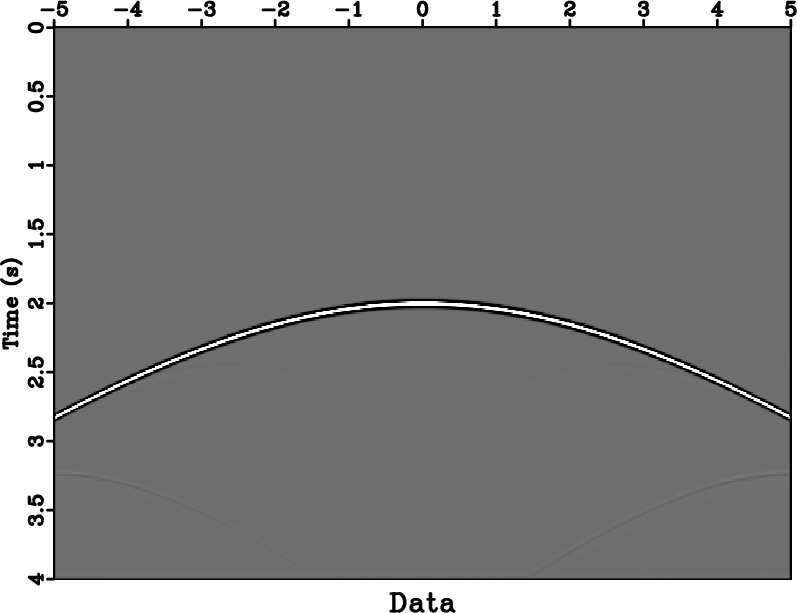
\includegraphics[scale=0.3]{/home/vgolubev/work/github/acinverse/madagascar/report/Fig/Figure_1.png}
}
\captionof{figure}{Сейсмограмма с одной прямой границей.}
\label{seismo_1}
\end{minipage}

Также имеется возможность построения Zero-Offset сейсмограммы, т.е. когда каждая сейсмотрасса получена в условиях совпадения координат источника и приёмника.
На рисунке \ref{seismo_2} показана ZO-сейсмограмма для той же самой модели среды.
Использовался 2001 источник-приёмник с интервалом 50 м на всё протяжении расчётной области.

\noindent
\begin{minipage}{\linewidth}
\makebox[\linewidth]{
  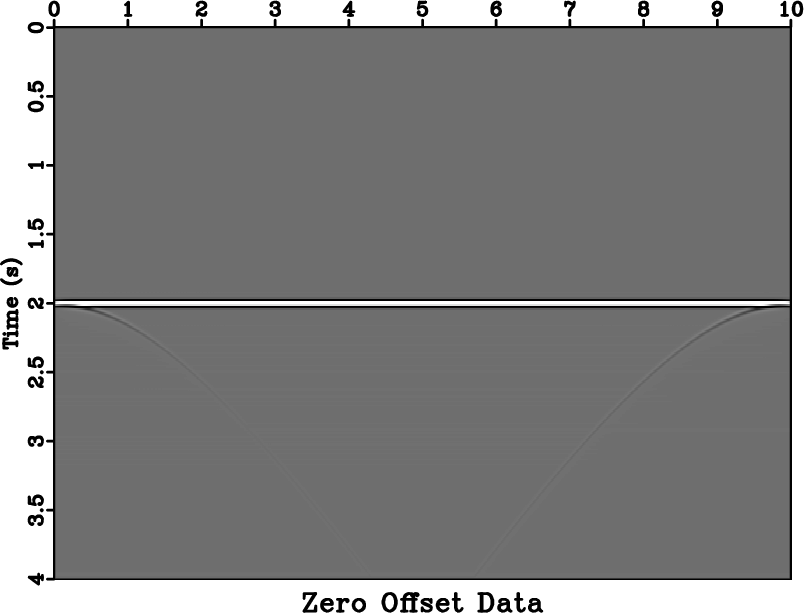
\includegraphics[scale=0.3]{/home/vgolubev/work/github/acinverse/madagascar/report/Fig/Figure_2.png}
}
\captionof{figure}{ZO-cейсмограмма с одной прямой границей.}
\label{seismo_2}
\end{minipage}

При этом программа kirmod позволяет получить синтетическую сейсмограмму для произвольного распределения отражающих границ в пространстве.
Их можно задавать аналитическими функциями.
Для примера была рассчитана модель среды с тремя отражающими горизонтами, два из которых криволинейные.
Границы задавались функциями $x_2 = (3.0 - 0.1 * x_1)$, $x_2 = 0.5 * e^{\frac{(x_1 - 5.0)^2}{25}} - 0.4$ и $x_2 = -3.8 + 0.1 * x_1 + e^{\frac{(x_1 - 5.0)^2}{25}}$ соответственно.
При этом обозначены $x_1$ - горизонтальная ось, $x_2$ - вертикальная ось.
Параметры расстановки выбирались аналогично предыдущему расчёту.
Результаты расчётов представлены на рисунках \ref{seismo_3} - \ref{seismo_4}.

\noindent
\begin{minipage}{\linewidth}
\makebox[\linewidth]{
  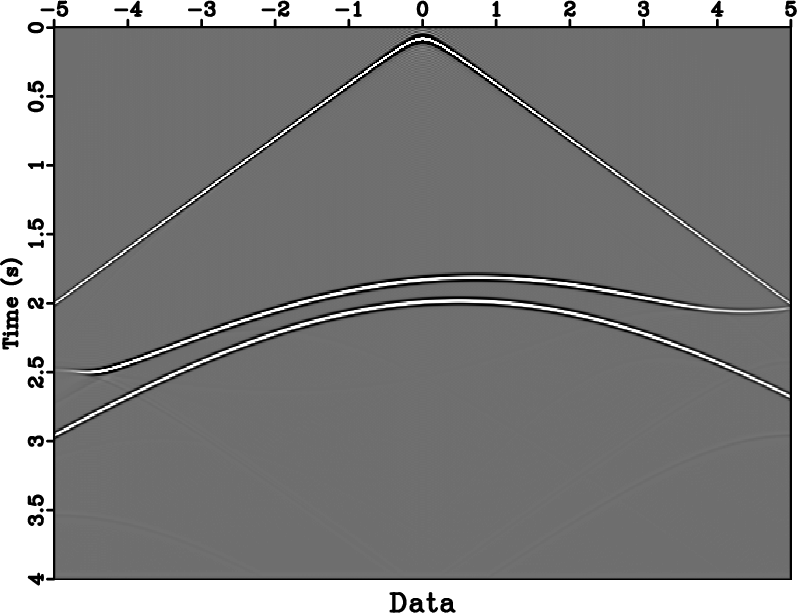
\includegraphics[scale=0.3]{/home/vgolubev/work/github/acinverse/madagascar/report/Fig/Figure_3.png}
}
\captionof{figure}{Сейсмограмма для модели с тремя отражающими горизонтами.}
\label{seismo_3}
\end{minipage}

\noindent
\begin{minipage}{\linewidth}
\makebox[\linewidth]{
  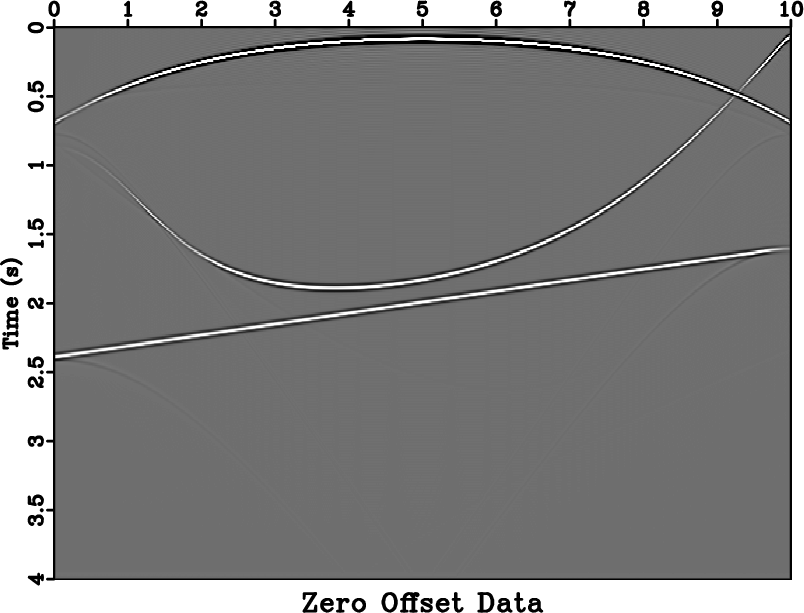
\includegraphics[scale=0.3]{/home/vgolubev/work/github/acinverse/madagascar/report/Fig/Figure_4.png}
}
\captionof{figure}{ZO-сейсмограмма для модели с тремя отражающими горизонтами.}
\label{seismo_4}
\end{minipage}

\subsection{Миграция. Интеграл Кирхгофа.}

Рассмотрим простейший случай, когда расчётная сетка кубическая, и на поверхности сейсмоприёмники расположены в каждом её узле.
В таком случае формула (\ref{rayleigh_migration}) может быть записана в виде:
\begin{equation}
\label{rayleigh_migration_discrete}
U^m(i,j,k) = -\frac{1}{2\pi}\frac{\sum\limits_{l,m} \frac{U(l,m,\frac{2d(i,j,k+1,l,m)}{c})}{d(i,j,k+1,l,m)}\delta x \delta y - \sum\limits_{l,m} \frac{U(l,m,\frac{2d(i,j,k,l,m)}{c})}{d(i,j,k,l,m)}\delta x \delta y}{\delta z},
\end{equation}
где $d(i,j,k,l,m)=\sqrt{(l-i)^2(\delta x)^2 + (m-j)^2(\delta y)^2  + (k)^2(\delta z)^2}$, а начало координат находится в точке $(i,j,k)=(0,0,0)$.

Была реализована программа AcInverse на языке C++, производящая миграцию Кирхгофа (Рэлея).
Для её тестирования были использованы сейсмограммы, генерируемые ПО Madagascar для различного расположения отражающих границ.

\todo[inline]{ПРИМЕРЫ МИГРАЦИИ СО СЛОЖНЫМИ ГРАНИЦАМИ КИРХГОФОМ}

\subsection{Миграция. Приближение Борна.}

\todo[inline]{ОПИСАНИЕ ОТ ОЛЕГА ЧИСЛЕННОЙ РЕАЛИЗАЦИИ И РАСЧЁТОВ ПО БОРНУ}

\subsection{Сравнительный анализ двух алгоритмов миграции (Кирхгоф, Борн) на простых моделях}

Одной из целей работы являлось сравнение двух методов миграции (Кирхгоф и присоединённый оператор), реализованных в программах AcInverse и Borni.
Исследовалась 2D модель с двумя отражающими горизонтами\footnote{При расчёте сейсмограммы в Borni отражающие границы образовывались как результат включения одной большой неоднородности с $\delta s = 4*10^{-6}$}, которые задавались формулами:
\begin{itemize}
\item $z=-2$,
\item $z=-2 + (0.1 * x + 0.5)$.
\end{itemize}
Фоновая скорость распространения продольных волн 2500 м/с, геометрия расчётной области 10 км x 5 км.
Временная функция источника - Риккер с основной частотой 25 Гц.
В измерительную систему входил 201 источник и 201 приёмник, установленные каждые 50 м.

На рисунке \ref{seismo_verif_zo_madagascar_borni} (слева) приведена Zero-Offset-сейсмограмма, рассчитанная методом Кирхгофа (Madagascar, kirmod), а справа - программой Borni.
Как видно, Кирхгоф дал более чёткое изображение, хотя и с наличием сферических артефактов у границ области.
Таким образом, для тестирования алгоритмов миграции было получено два набора входных данных разными методами.

\noindent
\begin{minipage}{\linewidth}
\makebox[\linewidth]{
\begin{tabular}{cc}
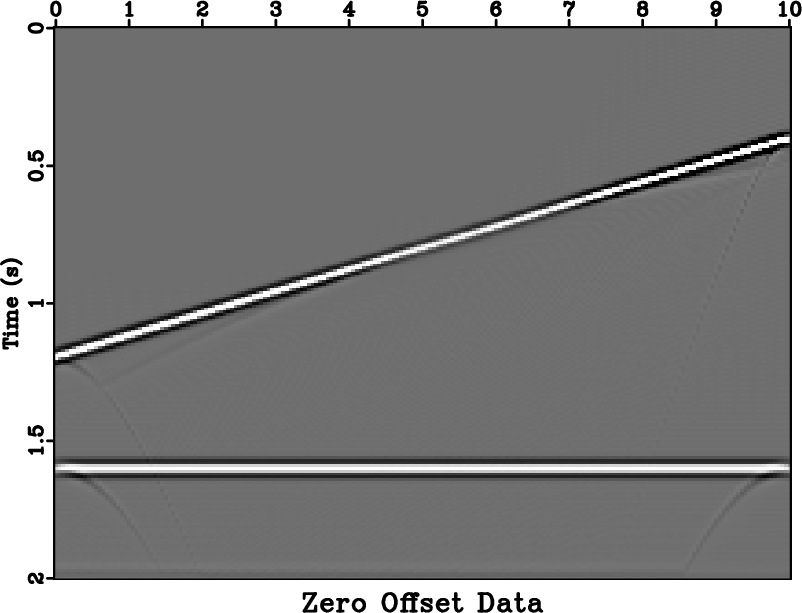
\includegraphics[width=50mm]{/home/vgolubev/work/github/acinverse/madagascar/report/Fig/seismo_verif_zo_madagascar_borni-madagascar.png}
&
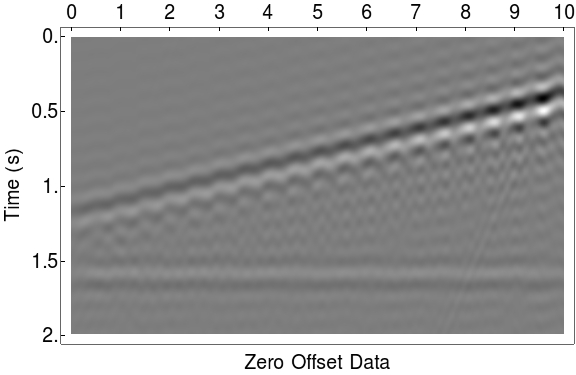
\includegraphics[width=60mm]{/home/vgolubev/work/github/acinverse/borni/seismo_verif_zo_madagascar_borni-borni.png}
\end{tabular}
}
\captionof{figure}{ZO-сейсмограмма для верификационной модели. Слева - Madagascar, справа - Borni.}
\label{seismo_verif_zo_madagascar_borni}
\end{minipage}

На рисунке \ref{seismo_verif_madagascar_borni-acinverse} представлены миграционные изображения, полученные методом Кирхгофа (AcInverse).
Можно говорить о выделяемости контактных границ, пусть и с небольшим контрастом и наличием артефактов.

\noindent
\begin{minipage}{\linewidth}
\makebox[\linewidth]{
  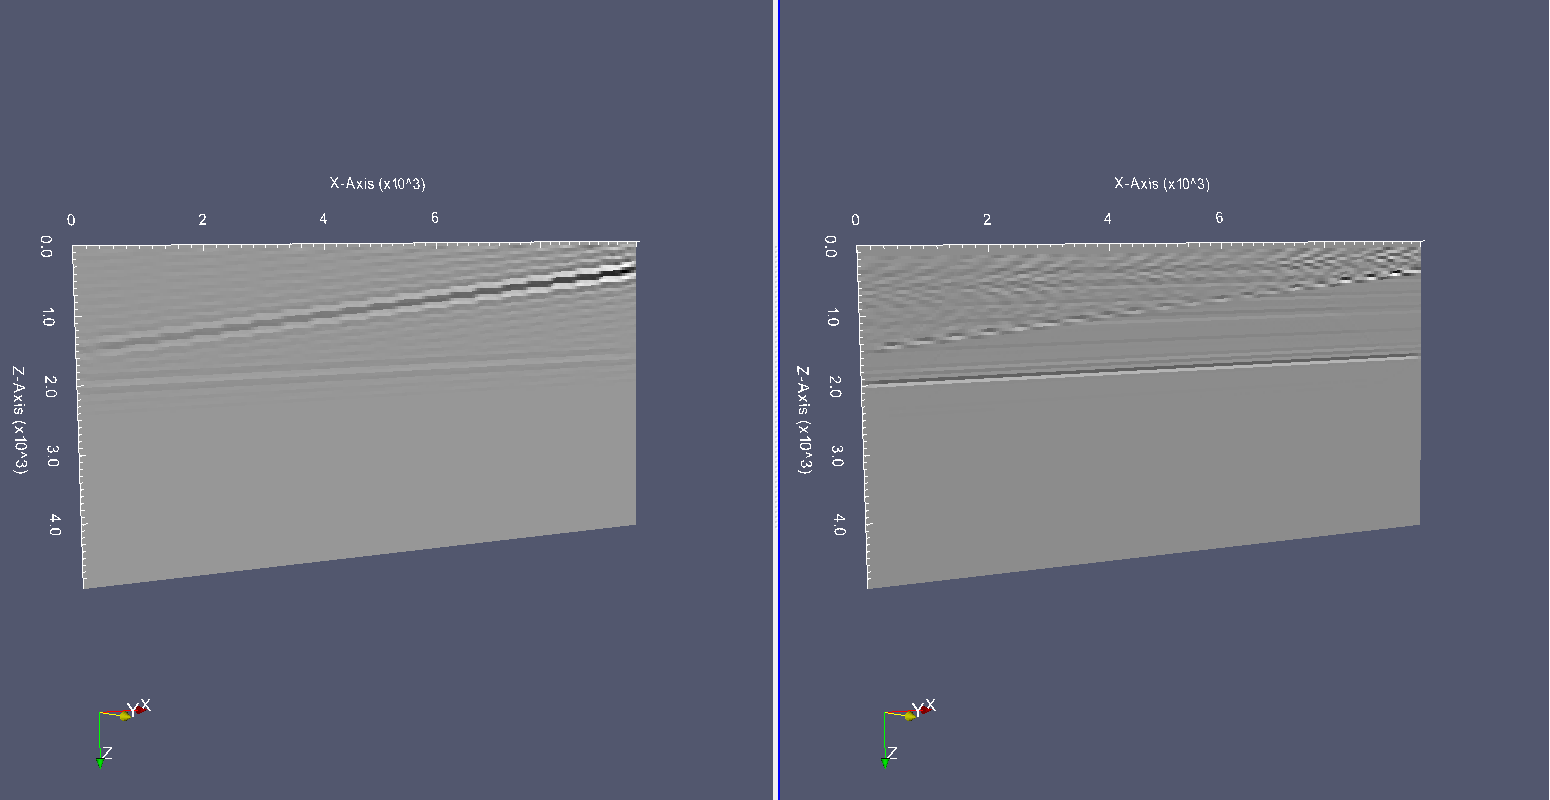
\includegraphics[width=100mm]{/home/vgolubev/work/github/acinverse/madagascar/report/Fig/seismo_verif_madagascar_borni-acinverse.png}
}
\captionof{figure}{Миграционное изображение для верификационной модели, полученное методом Кирхгофа (AcInverse). Слева - на входе Борн (Borni), справа - на входе Кирхгоф (Madagascar).}
\label{seismo_verif_madagascar_borni-acinverse}
\end{minipage}

На рисунке \ref{seismo_verif_madagascar_borni-borni} представлены миграционные изображения, полученные методом присоединённого оператора (Борн, Borni).

\noindent
\begin{minipage}{\linewidth}
\makebox[\linewidth]{
  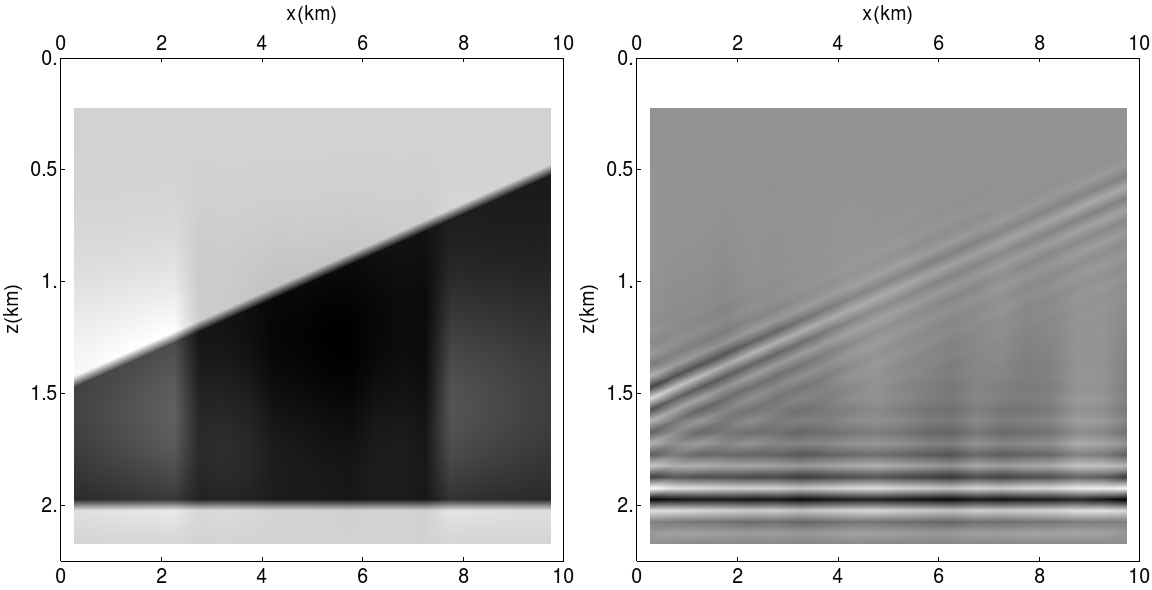
\includegraphics[width=120mm]{/home/vgolubev/work/github/acinverse/borni/seismo_verif_madagascar_borni-borni.png}
}
\captionof{figure}{Миграционное изображение для верификационной модели, полученное методом присоединённого оператора (Борн, Borni). Слева - на входе Борн (Borni), справа - на входе Кирхгоф (Madagascar).}
\label{seismo_verif_madagascar_borni-borni}
\end{minipage}

\section{Заключение}

\todo[inline]{ПЕРЕПИСАТЬ ЗАКЛЮЧЕНИЕ И ДАЛЬНЕЙШИЕ ПЛАНЫ}

В мартовский отчёт планируется включить приведённое выше сравнение методов миграции на трёхслойной модели в рамках задачи "Сравнительный анализ двух алгоритмов на простых моделях" и отдельные исследования (теория, чувствительность к параметрам) процедур миграции по Кирхгофу и Adjoint operator (Borne approximation).

Кроме того сформулированы направления дальнейшего исследования, с приоритетом которых нет чёткой определённости: 

\begin{enumerate}
\item Провести детальное исследование поведения алгоритмов миграции (AcInverse, Borni) при изменении расчётных параметров.
\item Провести верификационные сравнения таким же способом (К-К, Б-Б, К-Б, Б-К) на 2Д слоистых моделях с криволинейными границами, т.о. усложнив "простые модели".
\item Освоить в Madagascar решение прямой задачи FD методом (или доработать сеточно-характеристический метод), получить синтетическую ZO-сейсмограмму от верификационной трёхслойной модели и попробовать применить миграцию AcInverse и Borni.
\item Продлить границы 2Д модели вдоль третьей оси, чтобы получить 3Д, и провести верификационное тестирование на полученной 3Д модели.
\item Освоить Madagascar с целью построения ZO-сейсмограммы для сложной модели (например, Marmousi) и попробовать применить миграцию AcInverse и Borni.
\item Доработать Borni для реализации regularized least-square migration.
\item Перейти к построению матрицы L на основе finite-difference approximation, а потом реализовать аналог Borni на её основе.
\end{enumerate}

\section{Приложение 1. Пример построения матрицы L в приближении Борна}

Согласно теории, изложенной в \cite{Zhdanov_2007}, в акустическом приближении связь между наблюдаемым давлением на
сейсмоприёмниках на поверхности и параметрами среды может быть выражена следующей формулой (приближение Борна, \cite{Zhdanov_2007}, 15.5):

\begin{equation}
\label{eq_born_approximation_1}
p^s(\vec{r}_j, w) = w^2\int_D G^w_b(\vec{r}_j|\vec{r};w)\Delta s^2(\vec{r})p^i(\vec{r},w)  dv,
\end{equation}

в которой $\vec{r}_j$ - радиус-вектор точки приёмника, $D$ - область, в которой параметр медленности ($s = \frac{1}{c}$)
отличается от фоновой медленности ($s_b = \frac{1}{c_b},\Delta s^2 = \frac{1}{c^2} - \frac{1}{c^2_b})$, $p^i$ - давление, которое создавалось бы
в отсутствии неоднородности в области $D$, $G^w_b$ - функция Грина для фоновой медленности.
Для однородной среды функция Грина может быть записана в виде (\ref{eq_grin_function}).
Подставляя (\ref{eq_grin_function}) в формулу (\ref{eq_born_approximation_1}) получим:

\begin{equation}
\label{eq_born_approximation_2}
p^s(\vec{r}_j, w) = w^2\int_D \frac{1}{4\pi|\vec{r}-\vec{r}_j|}e^{iw\frac{|\vec{r}-\vec{r}_j|}{c_b}} \Delta s^2(\vec{r})p^i(\vec{r},w)  dv.
\end{equation}

Займёмся теперь вычислением $p^i$.
Пусть источник возмущения - точечный взрыв, происходящий в нулевой момент времени в точке $\vec{r}_0$.
Тогда в случае однородной среды с фоновой медленностью $s_b$ можно записать решение в виде:

\begin{equation}
\label{eq_point_explosion}
p^i(\vec{r}, w) = \frac{1}{4\pi|\vec{r}-\vec{r}_0|}e^{iw\frac{|\vec{r}-\vec{r}_0|}{c_b}}.
\end{equation}

Подставляя (\ref{eq_point_explosion}) в формулу (\ref{eq_born_approximation_2}) получим:

\begin{eqnarray}
\label{eq_born_approximation_3}
p^s(\vec{r}_j, w) = w^2\int_D \frac{1}{4\pi|\vec{r}-\vec{r}_j|}e^{iw\frac{|\vec{r}-\vec{r}_j|}{c_b}} \Delta s^2(\vec{r})\frac{1}{4\pi|\vec{r}-\vec{r}_0|}e^{iw\frac{|\vec{r}-\vec{r}_0|}{c_b}}  dv = \nonumber \\
= \frac{w^2}{16\pi^2} \int_D \frac{e^{iw\frac{|\vec{r}-\vec{r}_0| + |\vec{r}-\vec{r}_j|}{c_b}}}{|\vec{r}-\vec{r}_j||\vec{r}-\vec{r}_0|} \Delta s^2(\vec{r}) dv.
\end{eqnarray}

Вводя дискретизацию по пространству в виде параллелепипедной сетки с шагами $\delta x, \delta y, \delta z$ и индексами $l, m, p$ формулу (\ref{eq_born_approximation_3}) можно
привести к виду:

\begin{equation}
\label{eq_born_approximation_num}
p^s(\vec{r}_j, w) = \frac{w^2}{16\pi^2} \sum_{(l,m,p)\in D} \frac{e^{iw\frac{|\vec{r}_{l,m,p}-\vec{r}_0| + |\vec{r}_{l,m,p}-\vec{r}_j|}{c_b}}}{|\vec{r}_{l,m,p}-\vec{r}_j||\vec{r}_{l,m,p}-\vec{r}_0|} \Delta s_{l,m,p}^2 \delta x \delta y \delta z.
\end{equation}

На первом этапе рассмотрим двумерный случай, когда вдоль $Y$ содержится всего одна ячейка.
Тогда можно избавиться от индекса $m$, а также сейсмодатчики устанавливаются вдоль одной линии $OX$ и могут быть параметризованы одним индексом $j$.
Формула (\ref{eq_born_approximation_num}) сводится к виду:

\begin{equation}
\label{eq_born_approximation_num_2D}
p^s(x_j, w) = \frac{w^2 \delta x \delta z}{16\pi^2} \sum_{(l,p)\in D} \frac{e^{iw\frac{D_{l,p}+d_{j,l,p}}{c_b}}}{D_{l,p}d_{j,l,p}} \Delta s_{l,p}^2,
\end{equation}

где $D_{l,p}=|\vec{r}_{l,p}-\vec{r}_0|$ и $d_{j,l,p}=|\vec{r}_{l,p}-\vec{x}_j|$.

Пусть матрица $\Delta s_{l,p}^2$ развернута в $1D$ массив так, что последовательно в нём лежат её строки.
И пусть размер модели по $X$ равен $P$, а по $Z$ - $L$.
Тогда индекс в массиве имеет вид $ind = p + l * P$, $p \in [0, P - 1], l \in [0, L - 1]$.
Также справедливы равенства: $l = [\frac{ind}{P}]$ и $p = ind - [\frac{ind}{P}] * P$.

С учётом введённой параметризации массива и того факта, что вне неоднородности $\Delta s^2 = 0$, можно записать формулу (\ref{eq_born_approximation_num_2D}) в виде:

\begin{equation}
\label{eq_born_approximation_num_2D_ind}
p^s(x_j, w) = \sum_{(ind)\in [0, L * P - 1]} L_{j,ind} \Delta s_{ind}^2,
\end{equation}

где матрица $L_{j,ind} = \frac{w^2 \delta x \delta z}{16\pi^2} \frac{e^{iw\frac{D_{ind}+d_{j,ind}}{c_b}}}{D_{ind}d_{j,ind}}$,
$D_{ind}=\sqrt{(x_{ind} - x_0)^2 + (y_{ind} - y_0)^2}$ и $d_{j,ind}=\sqrt{(x_{ind} - x_j)^2 + y_{ind}^2}$.
Это и является реализованным представлением зависимости данных на приёмниках от параметров модели.
При обобщении на трёхмерный случай усложнится лишь формула для вычисления значения $ind$, тогда как все остальные рассуждения не изменятся.

\bibliographystyle{acm}
\bibliography{report_April_1}

\end{document}
